\documentclass{article}%
\usepackage[T1]{fontenc}%
\usepackage[utf8]{inputenc}%
\usepackage{lmodern}%
\usepackage{textcomp}%
\usepackage{lastpage}%
\usepackage[head=40pt,margin=0.5in,bottom=0.6in]{geometry}%
\usepackage{graphicx}%
%
\title{\textbf{Denuncian que Rubén González fue torturado en La Pica}}%
\author{Carlos Seijas Meneses}%
\date{02/12/2018}%
%
\begin{document}%
\normalsize%
\maketitle%
\textbf{URL: }%
http://www.el{-}nacional.com/noticias/presos{-}politicos/denuncian{-}que{-}ruben{-}gonzalez{-}fue{-}torturado{-}pica\_261811\newline%
%
\textbf{Periodico: }%
EN, %
ID: %
261811, %
Seccion: %
Presos políticos\newline%
%
\textbf{Palabras Claves: }%
Presos políticos\newline%
%
\textbf{Derecho: }%
1.2%
, Otros Derechos: %
1.3, 2.3%
, Sub Derechos: %
1.2.2, 1.3.1, 2.3.3%
\newline%
%
\textbf{EP: }%
NO\newline%
\newline%
%
\textbf{\textit{Dirigentes sindicales aseguran que el trabajador pasó la noche esposado de pies y manos, en el suelo de un pasillo de la cárcel}}%
\newline%
\newline%
%
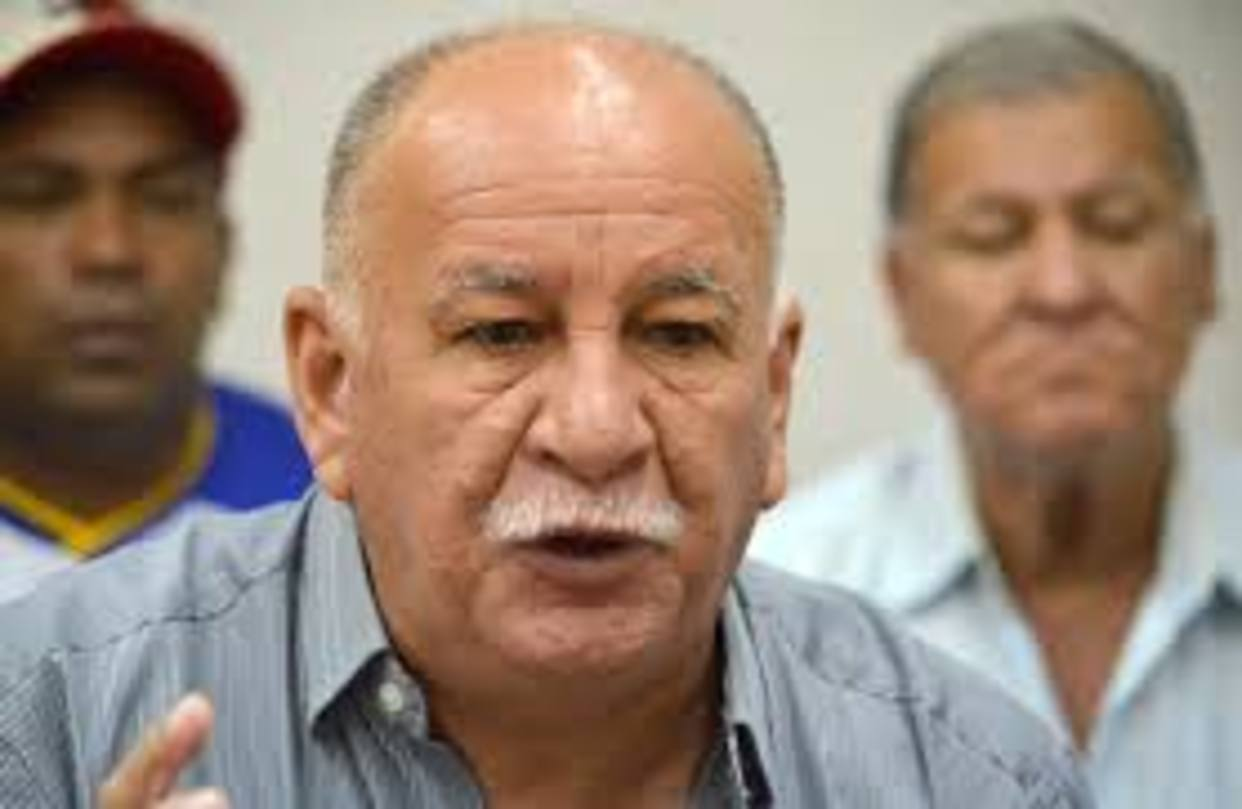
\includegraphics[width=300px]{187.jpg}%
\newline%
%
Esposado de pies y manos en el suelo de un pasillo de la cárcel de La Pica pasó la noche Rubén González, secretario general del Sindicato de Ferrominera.%
\newline%
%
Fue horas después cuando enfrente de familiares y trabajadores, que tuvieron acceso a la prisión, funcionarios de la GNB le quitaron las esposas y supuestamente lo llevaron al médico forense, dijo Pablo Zambrano, secretario ejecutivo de Fetrasalud. “Una vez más Nicolás Maduro viola los derechos humanos. Cuando un gobierno permite ese tipo de cosas, vemos el talante antidemocrático. No le importa torturar a un ciudadano. Rubén es cualquiera de nosotros, cualquier persona que levanta la voz”, expresó.%
\newline%
%
Juan Véliz, presidente del Sindicato de Cantv, denunció: “Rubén González ha sido objeto de un trato inhumano en La Pica, donde estuvo esposado y tirado en el piso como un animal”.%
\newline%
%
El jueves en la madrugada, guardias nacionales detuvieron a González después de que en Anaco retuvieron a 60 trabajadores de empresas básicas de Guayana, entre ellos al dirigente sindical, que regresaban de una protesta realizada el miércoles en Caracas. El viernes en la noche un tribunal militar de Maturín, Monagas, dictó privativa de libertad contra González y ordenó su reclusión en la cárcel de La Pica.~Le fueron imputados tres cargos militares: ataque al centinela, ultraje al centinela y ultraje a la FANB.%
\newline%
%
“No dejaremos de reclamar y también nos corresponde defender a todos los compañeros que están presos en El Dorado”, dijo Zambrano. El martes en la mañana funcionarios de la DGCIM detuvieron a Douglas Álvarez, Yonney Monsalve, Alexis Perdomo, Exddy Perdomo, Francisco Perdomo, Pedro Calzadilla, Argenis Dasilva, Tony Briceño y a José Jaime que protestaban en el portón IV de la empresa. El jueves en la tarde fueron trasladados a las colonias móviles de El Dorado.%
\newline%
%
La dirigente Marlene Sifontes, secretaria de Organización de Sunep{-}Inparques, afirmó que la Intersectorial de Trabajadores se mantiene en reunión permanente desde la detención “arbitraria” de González, para coordinar acciones de lucha y exigir la libertad de los compañeros “secuestrados”.%
\newline%
%
Marcela Máspero, presidente de Únete, afirmó que la Comisión de Encuesta, presidida por Manuel Herrera Carbuccia, ya acusó recibo de las denuncias que envió Únete el jueves en la noche, en la que solicitan a Guy Ryder, director general de la Organización Internacional del Trabajo, “protección expresa para todos los dirigentes de Venezuela ante la arremetida de los cuerpos parapoliciales del gobierno, que de forma violenta agreden e interfieren en las protestas en pro de nuestras conquistas”.%
\newline%
%
\end{document}